\section{Evaluation}
\label{Eva}

In this section, we describle our performance evaluation in real-scene
experiments. We distribute 130 TI SensorTag sensors in an about $250~\times~250$
square meters area, with contiki-ng as its operating system. We use different
metrics for various applications and compare our works with other
state-of-the-art works.

\subsection{Routing}
\textbf{Energy efficiency}

We estimate sensor energy cost by multipling different coefficients on CPU
running time and radio listening and transmitting time and summing them up. The
coefficients are proportional to the working current described in sensor's
DataSheet.

\begin{figure}[htbp]
	\centering
	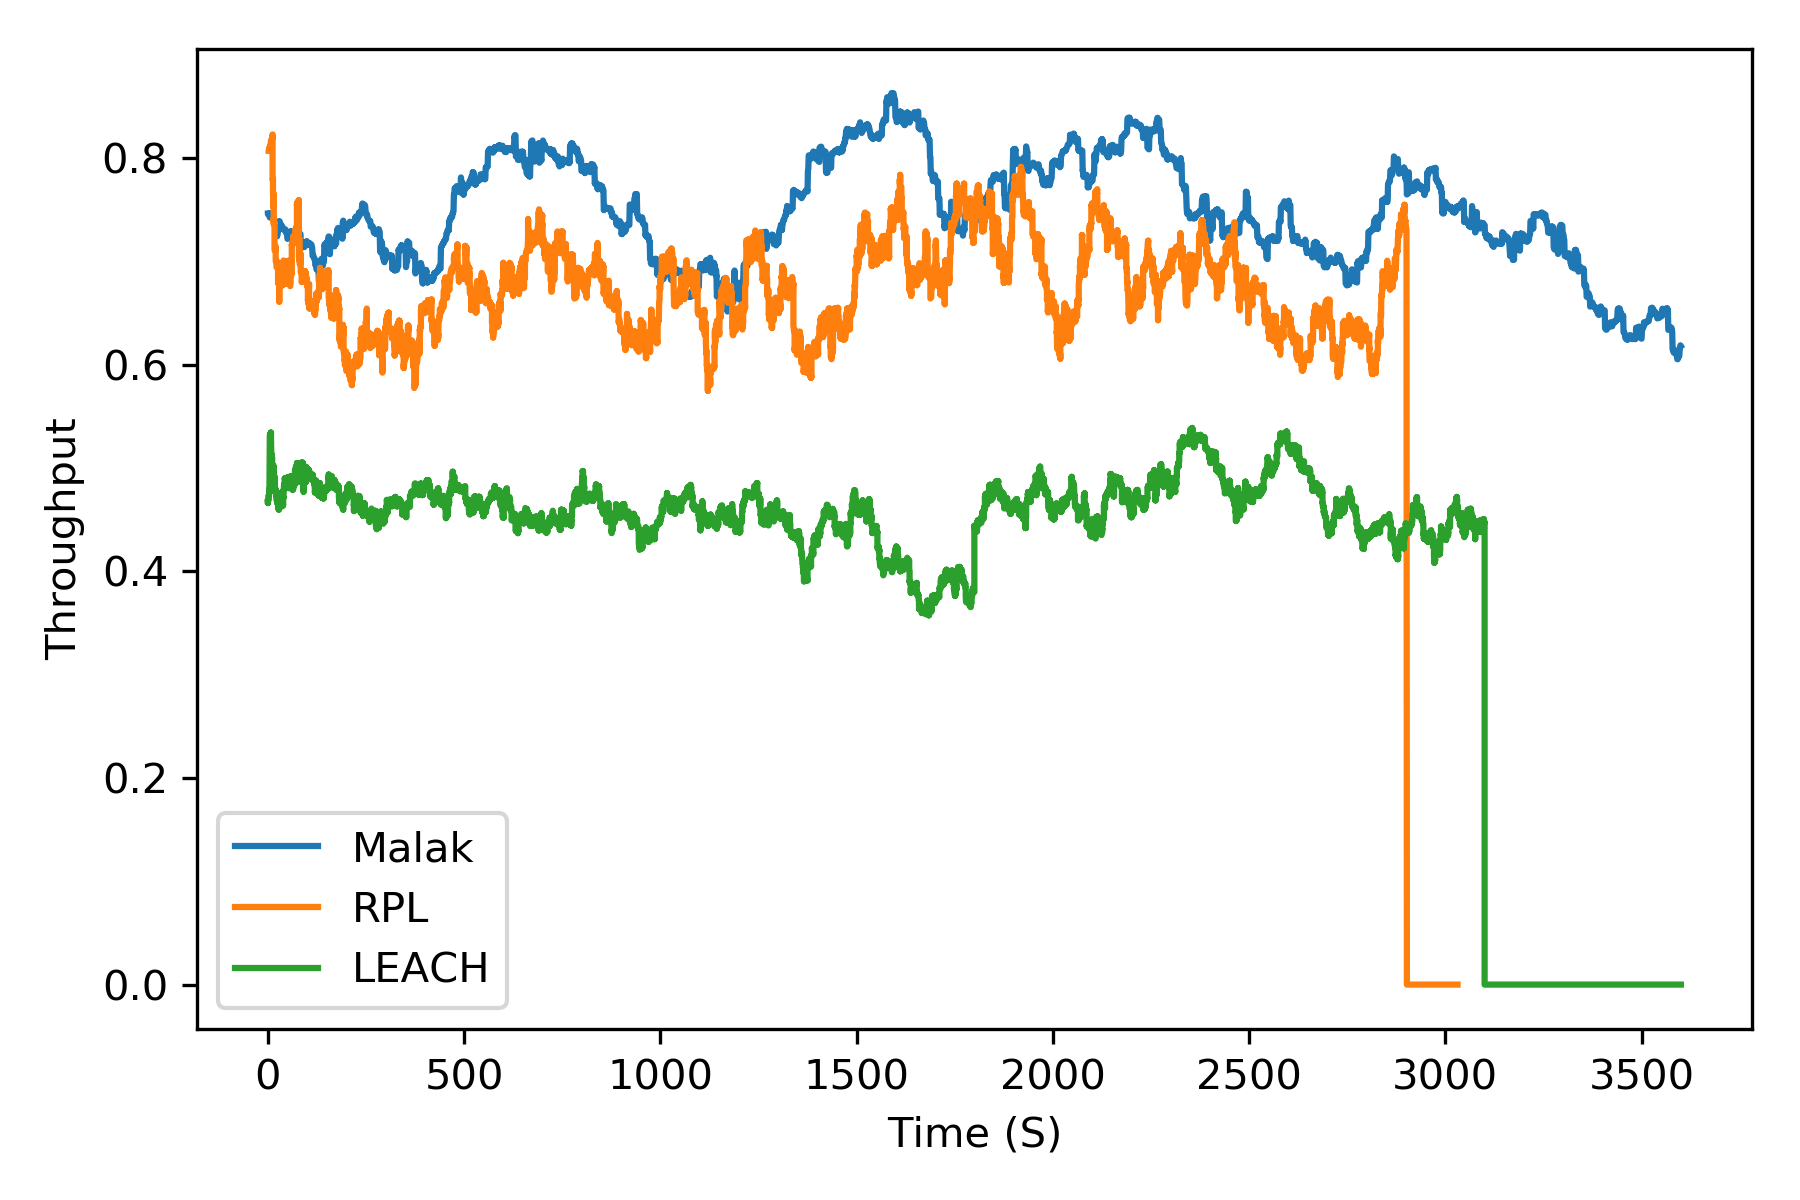
\includegraphics[width=.85\columnwidth]{Figure/throughput}
	\vspace{-0.1in}
	\caption{Routing throughput.
		\textnormal{The figure shows throughput
			corresponding to three kinds of Routing algorithms. Throughput can
			drop to zero when some key nodes are dead in the network.}}
	\label{throughput}
	\vspace{-0.2in}
\end{figure}

\textbf{Fault-tolerance}

\textbf{Scalability}

\subsection{Network Diagnosis}
\textbf{Robustness}

\subsection{AI Node Selection}
\textbf{Scalability}

\subsection{AI Energy Prediction}
\textbf{Prediction accuracy}

\begin{figure}[htbp]
	\hspace{-0.3cm}
	\centering
	\subfloat[Energy prediction]{
		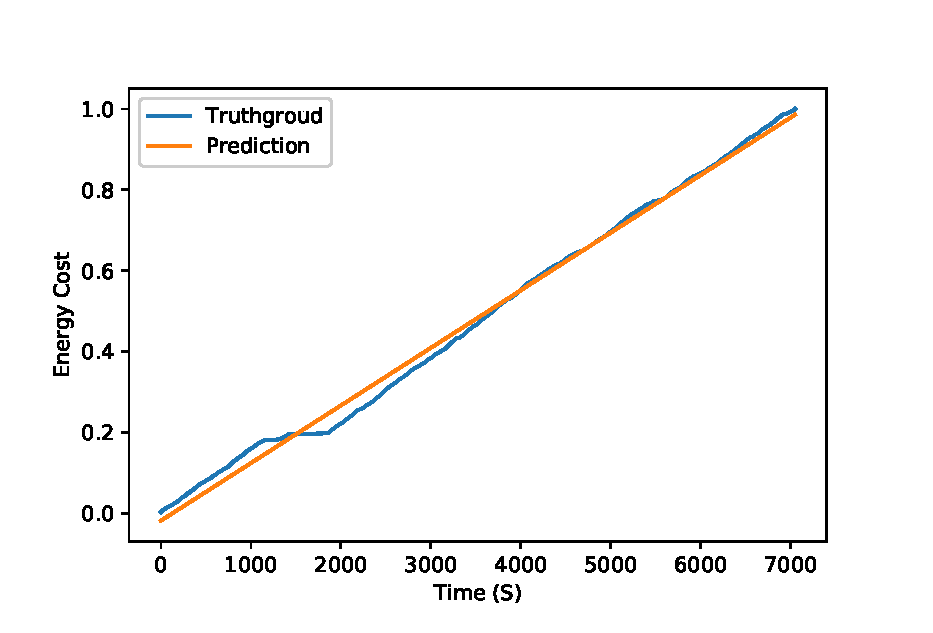
\includegraphics[width=.43\columnwidth]{Figure/energy_pred}
		\label{energy_pred:a}
	}
	\hspace{0.3cm}
	\subfloat[Energy prediction error]{
		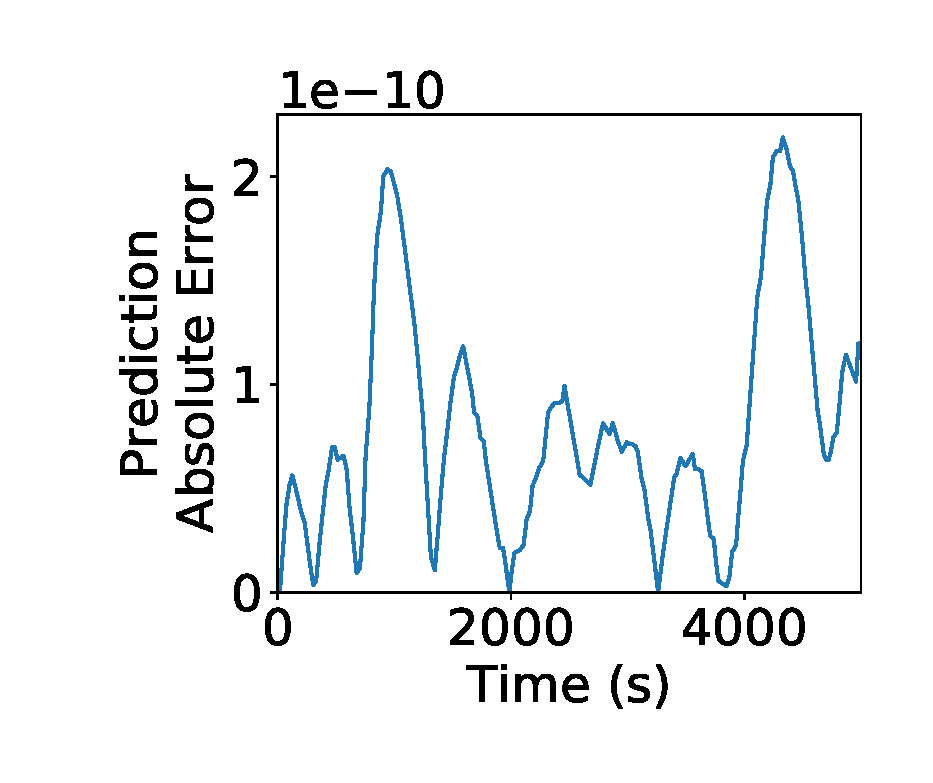
\includegraphics[width=.43\columnwidth]{Figure/energy_pred_err}
		\label{energy_pred:b}
	}
	\vspace{-0.1in}
	\caption{Energy prediction
		\textnormal{
			We use regression method to predict energy consumption and the
			prediction result is consistent with the truthground.  The absolute
			error of energy prediction never exceeds 0.05 with normalized energy
			(i.e. the maximum energy of a sensor is 1).
		}
	}
	\label{energy_pred}
	\vspace{-0.1in}
\end{figure}

\subsection{Multi-tasks}
\textbf{Energy Performance}
\textbf{Scalability}
\begin{figure}[htbp]
	\centering
	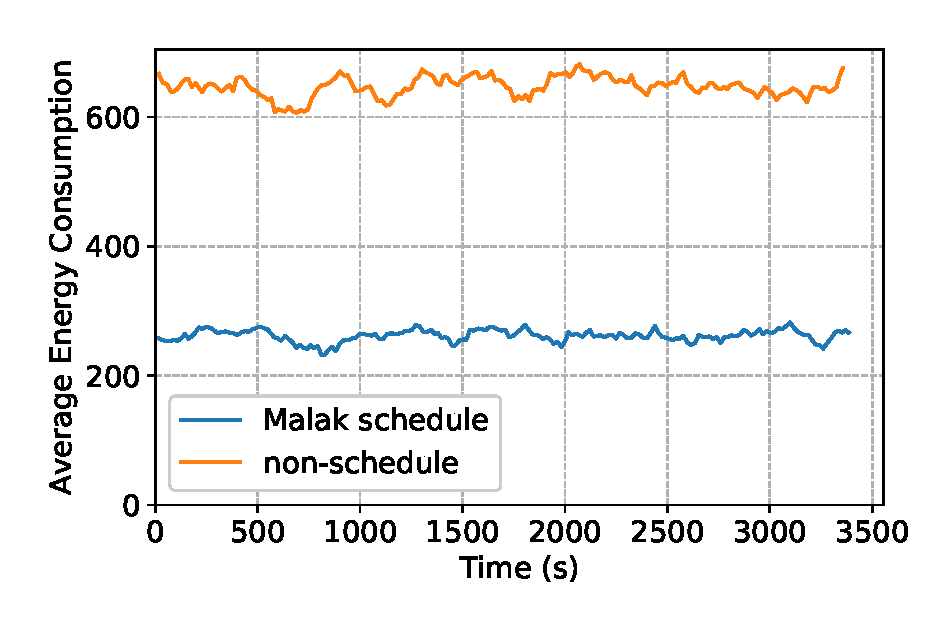
\includegraphics[width=.85\columnwidth]{Figure/multitask_energy}
	\vspace{-0.1in}
	\caption{Average energy consumption with and without multitask schedule
		\textnormal{When with multitask schedule, sensor consumes half of the energy
			comparing to when without multitask schedule.}}
	\label{multitask_energy}
	\vspace{-0.2in}
\end{figure}
